
%% bare_jrnl_compsoc.tex
%% V1.4a
%% 2014/09/17
%% by Michael Shell
%% See:
%% http://www.michaelshell.org/
%% for current contact information.
%%
%% This is a skeleton file demonstrating the use of IEEEtran.cls
%% (requires IEEEtran.cls version 1.8a or later) with an IEEE
%% Computer Society journal paper.
%%
%% Support sites:
%% http://www.michaelshell.org/tex/ieeetran/
%% http://www.ctan.org/tex-archive/macros/latex/contrib/IEEEtran/
%% and
%% http://www.ieee.org/

%%*************************************************************************
%% Legal Notice:
%% This code is offered as-is without any warranty either expressed or
%% implied; without even the implied warranty of MERCHANTABILITY or
%% FITNESS FOR A PARTICULAR PURPOSE! 
%% User assumes all risk.
%% In no event shall IEEE or any contributor to this code be liable for
%% any damages or losses, including, but not limited to, incidental,
%% consequential, or any other damages, resulting from the use or misuse
%% of any information contained here.
%%
%% All comments are the opinions of their respective authors and are not
%% necessarily endorsed by the IEEE.
%%
%% This work is distributed under the LaTeX Project Public License (LPPL)
%% ( http://www.latex-project.org/ ) version 1.3, and may be freely used,
%% distributed and modified. A copy of the LPPL, version 1.3, is included
%% in the base LaTeX documentation of all distributions of LaTeX released
%% 2003/12/01 or later.
%% Retain all contribution notices and credits.
%% ** Modified files should be clearly indicated as such, including  **
%% ** renaming them and changing author support contact information. **
%%
%% File list of work: IEEEtran.cls, IEEEtran_HOWTO.pdf, bare_adv.tex,
%%                    bare_conf.tex, bare_jrnl.tex, bare_conf_compsoc.tex,
%%                    bare_jrnl_compsoc.tex, bare_jrnl_transmag.tex
%%*************************************************************************


% *** Authors should verify (and, if needed, correct) their LaTeX system  ***
% *** with the testflow diagnostic prior to trusting their LaTeX platform ***
% *** with production work. IEEE's font choices and paper sizes can       ***
% *** trigger bugs that do not appear when using other class files.       ***                          ***
% The testflow support page is at:
% http://www.michaelshell.org/tex/testflow/


\documentclass[10pt,conference,onecolumn,compsoc]{IEEEtran}


\usepackage{hyperref}
\usepackage{enumitem}
\setlist[itemize]{leftmargin=3 cm}
\setlist[enumerate]{leftmargin=3cm}



% *** CITATION PACKAGES ***
%
\ifCLASSOPTIONcompsoc
  % IEEE Computer Society needs nocompress option
  % requires cite.sty v4.0 or later (November 2003)
  \usepackage[nocompress]{cite}
\else
  % normal IEEE
  \usepackage{cite}
\fi
% cite.sty was written by Donald Arseneau
% V1.6 and later of IEEEtran pre-defines the format of the cite.sty package
% \cite{} output to follow that of IEEE. Loading the cite package will
% result in citation numbers being automatically sorted and properly
% "compressed/ranged". e.g., [1], [9], [2], [7], [5], [6] without using
% cite.sty will become [1], [2], [5]--[7], [9] using cite.sty. cite.sty's
% \cite will automatically add leading space, if needed. Use cite.sty's
% noadjust option (cite.sty V3.8 and later) if you want to turn this off
% such as if a citation ever needs to be enclosed in parenthesis.
% cite.sty is already installed on most LaTeX systems. Be sure and use
% version 5.0 (2009-03-20) and later if using hyperref.sty.
% The latest version can be obtained at:
% http://www.ctan.org/tex-archive/macros/latex/contrib/cite/
% The documentation is contained in the cite.sty file itself.



% *** GRAPHICS RELATED PACKAGES ***
%
\ifCLASSINFOpdf
   \usepackage[pdftex]{graphicx}
 
\else
 
\fi
% graphicx was written by David Carlisle and Sebastian Rahtz. It is
% required if you want graphics, photos, etc. graphicx.sty is already
% installed on most LaTeX systems. The latest version and documentation
% can be obtained at: 
% http://www.ctan.org/tex-archive/macros/latex/required/graphics/
% Another good source of documentation is "Using Imported Graphics in
% LaTeX2e" by Keith Reckdahl which can be found at:
% http://www.ctan.org/tex-archive/info/epslatex/
%
% latex, and pdflatex in dvi mode, support graphics in encapsulated
% postscript (.eps) format. pdflatex in pdf mode supports graphics
% in .pdf, .jpeg, .png and .mps (metapost) formats. Users should ensure
% that all non-photo figures use a vector format (.eps, .pdf, .mps) and
% not a bitmapped formats (.jpeg, .png). IEEE frowns on bitmapped formats
% which can result in "jaggedy"/blurry rendering of lines and letters as
% well as large increases in file sizes.
%
% You can find documentation about the pdfTeX application at:
% http://www.tug.org/applications/pdftex









% *** PDF, URL AND HYPERLINK PACKAGES ***
%
\usepackage{url}
% url.sty was written by Donald Arseneau. It provides better support for
% handling and breaking URLs. url.sty is already installed on most LaTeX
% systems. The latest version and documentation can be obtained at:
% http://www.ctan.org/tex-archive/macros/latex/contrib/url/
% Basically, \url{my_url_here}.




\begin{document}

\title{Calender App
%
%

% received ..."  text while in non-compsoc journals this is reversed. Sigh.

\author{Jeremy Gordon\\ Kyle Byassee% <-this % stops a space
}
}
\IEEEtitleabstractindextext{%
\begin{abstract}
Our group project is a calender application that runs in the background. Some of the functions are notifying the user of events, importing and exporting user profiles and customizing the user experience with pictures. The target audience are users that want more freedom from their calendar application. 
\end{abstract}

}


% make the title area
\maketitle



\IEEEdisplaynontitleabstractindextext

\IEEEpeerreviewmaketitle



\section{Introduction}

Our group project is a calender application, it will be built in a C\# WPF application that runs in the background. Some of the functions are notifying the user of events, view historic information and customizing the user experience with pictures. We are targeting individuals who want the ability to customize, export, import and set specific day/month/year/time notifications. 
We want to give the user a calendar application that better then what is offered currently.

\subsection{Background}
We decided on this project because we do not have much experience in C\#. We also felt we could improve on the traditional calender application providing additional freedom and features. Providing features like viewing historic information and customizing backgrounds with user pictures. A calender application sounded like a project that could be fun, challenging and a worthwhile semester long project.

\subsection{Impacts}

The project is geared towards a general audience. Our application is appealing to that audience because of the ability to view historic information, customize the look of the applications background, set custom notifications. It may have a small but positive effect on the end user helping manage and organize life events.

\subsection{Challenges}

The layout of the GUI seems daunting since some months have more days than others. We plan to take inspiration from the numerous calender application that are already in the wild. While also improving on the GUI layout making it more user friendly and intuitive.

Adjusting the GUI for events like leap years. - We plan on using already built time/date functions to account for this.


\section{Scope}
The app will display the current date and time when first opened. Let the user change the date and set a notification on that date at a specific time. The user should be able to set the background of the app to a designated picture format. The app should have important holidays and dates displayed. 

\subsubsection{Stretch-Goals}
Export a user profile to be imported later into the same or different calender application.
Adding weather to be displayed in the GUI of the application.

\subsection{Requirements}
The functional and non-functional requirements were gathered based upon what the program would need to be considered complete.

\subsubsection{Functional}
\begin{itemize}
\item User needs to be able to specify a specific day/month/year to add a notification.
\item User can change background of the calendar with a picture.
\item User can change and navigate through the month, year and day.
\item User can cancel or modify an existing notification.
\end{itemize}

\subsubsection{Non-Functional}
\begin{itemize}
\item User saved notifications should be encoded to protect user data.
\end{itemize}

\subsection{Use Cases}

\ref{tab:useCaseIndex}.




\begin{table}
\centering
\begin{tabular}{|c|c|c|c|c|}
\hline
Use Case ID & Use Case Name & Primary Actor & Complexity & Priority \\
\hline \hline
1 & Set a notification & User & Med & 1\\
\hline
\hline
2 & remove or change a set notification & User & Med & 1\\
\hline
3 & Change calender background & User & Low & 1\\
\hline
\hline
4 & View historic information & User & Low & 1\\
\hline

\end{tabular}
\caption{Sample use case table}
\label{tab:useCaseIndex}
\end{table}


\begin{itemize}
\item[Use Case Number:] 1-2
\item[Use Case Name:] Set a notification
\item[Description:] The user has a specific date and time they with for a notification to appear on. The user navigates to the desired date. Selects the date and then specifies a time where the program saves that data and creates a notification.
\end{itemize}

You will then go on to (minimally) discuss a basic flow for the process:

\begin{enumerate}
\item User navigates to desired date.
\item User selects the date.
\item User specifies a time on that date.
\item[Termination Outcome:] The user has a notification set on that time and day.
\end{enumerate}



Alternative: Notification has already been created
\begin{enumerate}
\item User navigates to the same date
\item User selects the date
\item User selects the same time
\item User chooses to cancel or modify existing notification
\item[Termination Outcome:] The notification has been modified or canceled
\end{enumerate}

\begin{itemize}
\item[Use Case Number:]3
\item[Use Case Name:] Change calender background
\item[Description:] The user desires to change the background of the calender 

\end{itemize}

\begin{enumerate}
\item User clicks on a button to upload an image.
\item User selects the image.
\item User confirms the selected image.
\item[Termination Outcome:] The user has change the background of the calender.
\end{enumerate}

\begin{itemize}
\item[Use Case Number:]4
\item[Use Case Name:] View historic information
\item[Description:] A user desires to view specific historic information on a date.

\end{itemize}

\begin{enumerate}
\item User navigates to a specific date.
\item User selects the specific date.
\item[Termination Outcome:] The historic information is displayed to the user.
\end{enumerate}



\subsection{Interface Mockups}
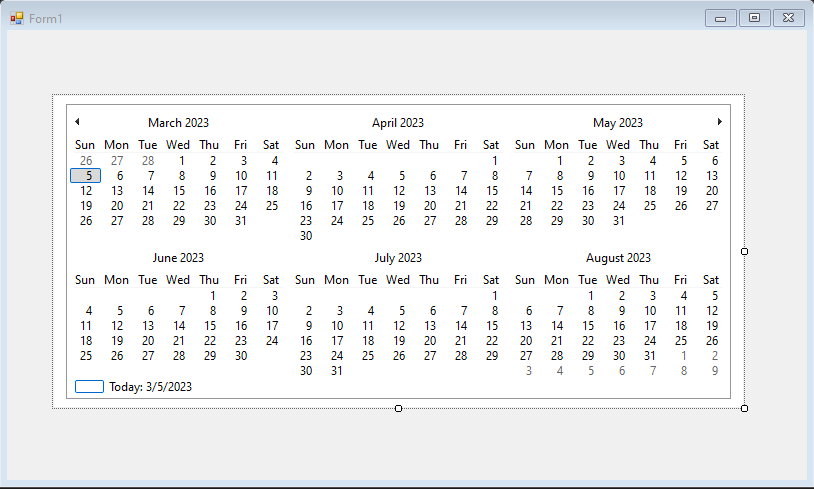
\includegraphics[height=250px, width=350px]{gui.png}
\break
\caption{Mockup of the GUI of our calender application}
\label{GUI Mockup}




\section{Project Timeline}
Go back to your notes and look up a typical project development life cycle for the Waterfall approach.  How will you follow this life cycle over the remainder of this semester?  This will usually involve a chart showing your proposed timeline, with specific milestones plotted out.  Make sure you have deliverable dates from the course schedule listed, with a plan to meet them (NOTE: these are generally optimistic deadlines).

\section{Project Structure}
At first, this will be a little empty (it will need to be filled in by the time you turn in your final report).  This is your chance to discuss all of your design decisions (consider this the README's big brother).

\subsection{UML Outline}
Show the full structure of your program.  Make sure to keep on updating this section as your project evolves (you often start out with one plan, but end up modifying things as you move along).  As a note, while Dia fails miserably at generating pdfs (probably my fault), I have had much success with png files.  Make sure to wrap your images in a \texttt{figure} environment, and to reference with the \texttt{ref} command.  For example, see Figure \ref{cat2}.

\begin{figure}[ht!]
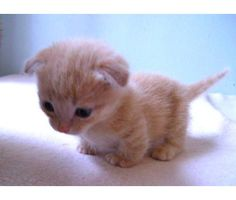
\includegraphics[scale=1.5]{cat2.jpg}
\caption{Your figures should be in the \emph{figure} environment, and have captions.  Should also be of diagrams pertaining to your project, not random internet kittens}
\label{cat2}
\end{figure}


\subsection{Design Patterns Used}
Make sure to actually use at least 2 design patterns from this class.  This is not normally part of such documentation, but largely just specific to this class -- I want to see you use the patterns!


\section{Results}
This section will start out a little vague, but it should grow as your project evolves.  With each deliverable you hand in, give me a final summary of where your project stands.  By the end, this should be a reflective section discussing how many of your original goals you managed to attain/how many desired use cases you implemented/how many extra features you added.

\subsection{Future Work}
Where are you going next with your project?
For early deliverables, what are your next steps?  (HINT: you will typically want to look back at your timeline and evaluate: did you meet your expected goals?  Are you ahead of schedule?  Did you decide to shift gears and implement a new feature?)
By the end, what do you plan on doing with this project?  Will you try to sell it?  Set it on fire?  Link to it on your resume and forget it exists?




\begin{thebibliography}{1}

\bibitem{IEEEhowto:kopka}
H.~Kopka and P.~W. Daly, \emph{A Guide to \LaTeX}, 3rd~ed.\hskip 1em plus
  0.5em minus 0.4em\relax Harlow, England: Addison-Wesley, 1999.

\end{thebibliography}



\begin{IEEEbiography}{Michael Shell}
Biography text here.
\end{IEEEbiography}

% if you will not have a photo at all:
\begin{IEEEbiographynophoto}{John Doe}
Biography text here.
\end{IEEEbiographynophoto}

% insert where needed to balance the two columns on the last page with
% biographies
%\newpage

\begin{IEEEbiographynophoto}{Jane Doe}
Biography text here.
\end{IEEEbiographynophoto}





% that's all folks
\end{document}


